In this section, we examine four potential issues with our analysis. We test an alternative responsiveness of government revenue to economic activity, different VAR orders, and whether the multiplier changes over time. 


\subsection{Government Revenue Response}

In our main analysis, we use a government revenue responsiveness to GDP changes of 1.7 based on \textcite{lutz2010fiscal}, which is different from the 2.08 value used in \textcite{blanchard2002empirical}. The 1.7 value is based on more updated data and methods, but we want to ensure this assumption is not driving all our results. Therefore, we estimate the model with $c_1 = 2.08$.

\begin{table}[t]
    \centering
    \caption{Estimated parameters and multiplier when $c_1 = 2.08$}
    \begin{tabular}{lcc}
    \toprule
    & (1) & (2) \\
    & $b_2 = 0$ & $c_2 = 0$ \\
    \midrule
    \emph{Parameters} \\
    \quad $a_1$ & -0.177 & -0.177 \\
    \quad $a_2$ & -0.163 & -0.163 \\
    \quad $b_2$ && 0.041 \\
    \quad $c_2$ & 0.919 \\
    \midrule
    \emph{Multiplier} \\
    \quad Estimate & 1.079 & 1.126 \\
    \quad Std. Err. & 0.115 & 0.115 \\
    \quad Time & 2 & 2 \\
    \bottomrule
\end{tabular}
    \label{tab:new-c1}
\end{table}

The results of this are in Table \ref{tab:new-c1}. The estimated parameters are almost identical to the earlier results in Table \ref{tab:results}. In both specifications, the $a_1$ and $a_2$ parameters are within 0.02 of those estimated earlier. The estimated multiplier is slightly higher, suggesting a 7-12\% multiplier effect, but still happens after a slight delay and is (almost) within a standard error of 1 where no multiplier effect exists.


\subsection{VAR Order}

The results in Section \ref{sec:results} use a fourth order VAR. We justify this choice using the taxation window that affects government revenue, but the causal effect should be robust to changes in the autoregressive order of the model. We test this by calculating the multiplier using a VAR with orders between 1 and 24, corresponding to a window between 1 quarter and 6 years.

\begin{figure}[t]
    \centering
    \caption{Estimated multiplier for different VAR orders}
    \begin{subfigure}{0.475\textwidth}
        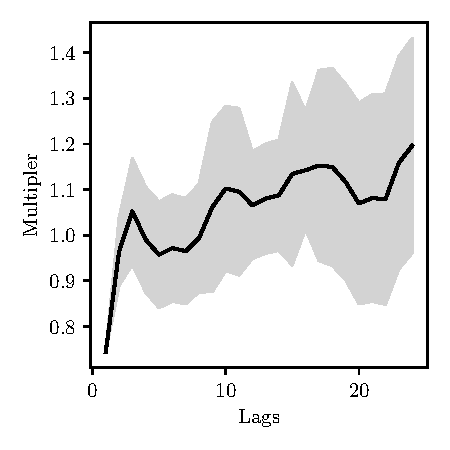
\includegraphics{figures/b20_lags.pdf}
        \caption{$b_2 = 0$}
    \end{subfigure}
    \begin{subfigure}{0.475\textwidth}
        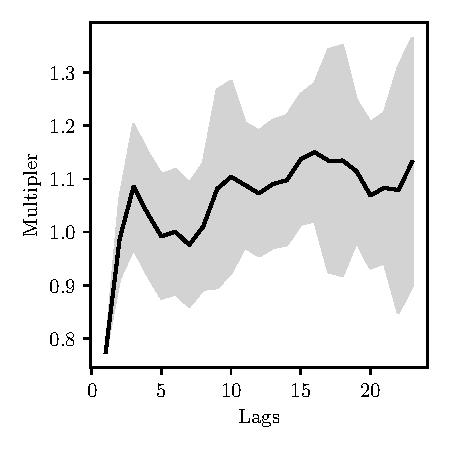
\includegraphics{figures/c20_lags.pdf}
        \caption{$c_2 = 0$}
    \end{subfigure}
    \label{fig:orders}
\end{figure}

The multiplier estimate for models with a different number of lags is shown in Figure \ref{fig:orders}. With only one lag, the estimate is much lower than our specification from Section \ref{sec:results} gets. However, the models that include more than one lag all estimate similar effects that are within the error interval of each other. Therefore, our order choice for the VAR does not determine our findings, and the causal effect is robust to different reasonable order choices.


\subsection{Temporal Trends in the Multiplier}

Our analysis in Section \ref{sec:results} assumes the multiplier is constant throughout the estimation window. We test this by estimating a separate multiplier for shorter periods within the estimation window. Specifically, we estimate the multiplier over a decade long period at 2.5-year intervals from 1947 to 2019. This extends the estimation window on both ends, so we also test the assumption that our multiplier estimates are meaningful after the estimation window, though that does mean the estimations are less meaningful during the 50s which had significantly larger government revenue and spending volatility and during estimation windows that include 2007 and 2008 due to the different growth trends during the period.

\begin{figure}[t]
    \centering
    \caption{Estimated multiplier for different estimation windows}
    \begin{subfigure}{0.475\textwidth}
        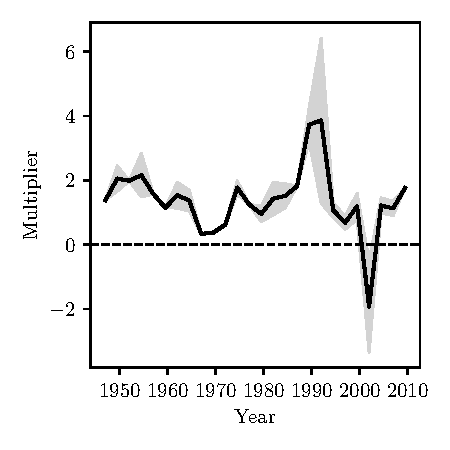
\includegraphics{figures/b20_ts.pdf}
        \caption{$b_2 = 0$}
    \end{subfigure}
    \begin{subfigure}{0.475\textwidth}
        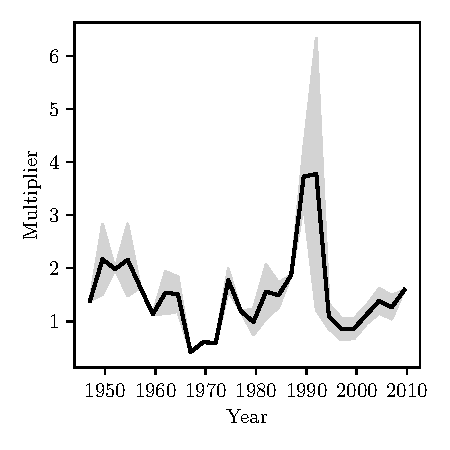
\includegraphics{figures/c20_ts.pdf}
        \caption{$c_2 = 0$}
    \end{subfigure}

    {\scriptsize \emph{Notes:} Multiplier calculated within a 10-year estimation windows that starts at the quarter on the x-axis.}
    \label{fig:ts}
\end{figure}

Figure \ref{fig:ts} shows the evolution of the multiplier over time. As expected, the estimates do not make sense in estimation windows that include 2007 and 2008 and are elevated pre-1960. Within the 1960 to 2007 estimation window, the multiplier hovers around our estimated value throughout most of the period, though does decrease in the late 60s and increase in the early 90s. Post-2008, the multiplier is near one in both specifications, suggesting our results could represent more recent business cycle forces. 
